
\documentclass[]{beamer}
\usetheme{PlasmaPhysics}
\usepackage{PlasmaPhysics}

\begin{document}

\begin{frame}

        \begin{center}
            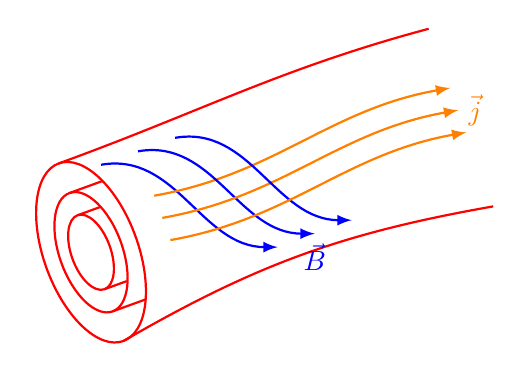
\begin{tikzpicture}[>=latex]
                \begin{scope}[rotate=20, red, thick]
                    \foreach \r in {0.5,0.8,1.2}{
                                        \draw (0,0) ellipse[x radius = 0.5*\r cm, y radius = \r cm];
                                    }
                                    \draw (0, 0.5) -- ++(0.3,0) (0, -0.5) -- ++(0.3,0);
                                    \draw (0, 0.8) -- ++(0.45,0) (0, -0.8) -- ++(0.45,0);
                                    \draw (0, 1.2) to[out=0, in=175] ++(5,0) (0, -1.2) to[out=10, in=170] ++(5,0);
                    \foreach \s in {1,2,3} {
                            \draw[->, blue] ({0.5*\s}, 1) to[out=-10, in=160] ++(1.75, -1.75) \ifnum\s=2 node[below] {$\vec{B}$} \fi;
                            \draw[->, orange] (1, {0.7-0.3*\s}) to[out=-10, in=170] ++(4, 0) \ifnum\s=2 node[right] {$\vec{j}$} \fi;
                        }
                \end{scope}
            \end{tikzpicture}
        \end{center}

0\end{frame}

\end{document}